\section{Design}

\begin{figure}[H]
    \centering
    \includegraphics[width=0.9\textwidth]{./images/fullscope1.PNG}
    \caption{Full-scope picture of the design }
    \label{fig:rfid1}
\end{figure}

The full-scope picture shows all connections in our design. The black dotted line is ground, yellow is 12V DC and red is 5V DC. Orange is used for data transfer. The 5V from the Arduino and D2 control the relay that opens for the 12V to the solenoid. There is a sensor in the lock that tells us when it is closed. That sends a signal to the Arduino in port D3. Ports A5 and A4 are connected to the LCD screen and it uses the $I^2 C$ protocol. Ports D9-D13 connects to the RFID reader using the UART protocol (Universal asynchronous receiver/transmitter).

\begin{figure}[H]
    \centering
    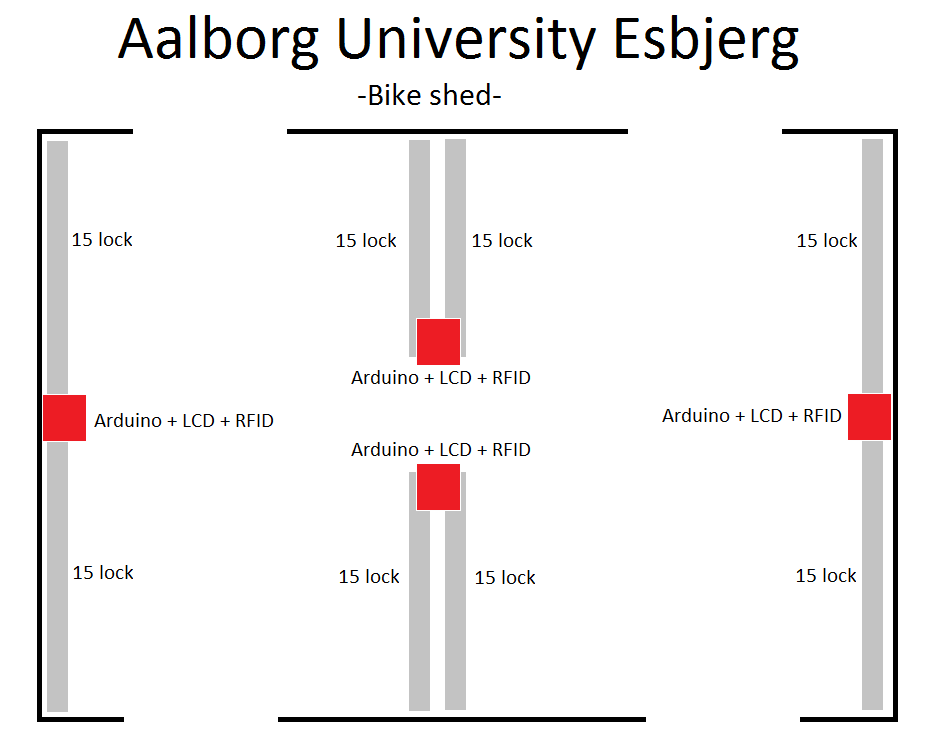
\includegraphics[width=0.5\textwidth]{./images/bikeshed.PNG}
    \caption{Aalborg University bike shed }
    \label{fig:bikeshed}
\end{figure}

Here is a basic concept idea of how we would implement the final design here in Aalborg University Esbjerg. For the final design a larger micro-controller would be necessary, like an Arduino MEGA, each MEGA could control up to 30 locks. All of the locks are controlled by a single RFID reader and one LCD screen. We would have our system on every other bicycle rack. So people could choose whether or not they wanted to use our system or their own locks. 

\subsection{Code}

\begin{figure}[H]
    \centering
    \includegraphics[width=1.1\textwidth]{./images/codeflow.PNG}
    \caption{Flowchart of the code used }
    \label{fig:codeflow}
\end{figure}

The flowchart shows a general idea of how our code will work. It will have two main functions. One is for locking new bicycles to the rack and the other is to unlock the bicycle. On the left side of the flowchart you can see a timer set t=30. If 30 seconds pass and no new RFID card is scanned to be associated with a lock, then the lock will automatically unlock. If a RFID card is read it will ignore to auto-unlock and continue with the program. 

\begin{algorithm}[H]
\caption{RFID bike lock}
\begin{algorithmic} 
\STATE LCD display - Welcome screen
\STATE
\WHILE{touch sensor pressed $= 1$}
\STATE sensor \textbf{X} = lock \textbf{X} 
\STATE LCD display - Is your lock number \textbf{X}? Then please read RFID card.
\STATE
\IF{RFID tag is valid}
\STATE lock \textbf{X} connects to RFID tag
\STATE timer $= 0$
\STATE LCD display - Bike lock \textbf{X} is now locked. Thank you
\STATE touch sensor pressed $= 0$
\ELSIF{RFID tag is invalid}
\STATE unlock bike lock \textbf{X}
\STATE LCD display - ERROR invalid or used card, Try again.
\ENDIF
\STATE
\IF{timer $= 30000$}
\STATE unlock bike lock \textbf{X}
\STATE LCD display - Bike lock \textbf{X} was not locked. Try again.
\ELSE
\STATE timer $=$ timer $+1$
\ENDIF
\STATE
\STATE delay $1$
\ENDWHILE
\STATE
\IF{RFID read}
\IF{RFID tag used}
\STATE unlock bike lock \textbf{X} that is connected to that card
\STATE LCD Display - Bike lock number \textbf{X} is now unlocked. Thank you.
\ELSE
\STATE LCD display - ERROR invalid or used card, Try again.
\ENDIF
\ENDIF
\end{algorithmic}
\end{algorithm}

\clearpage

\subsection{Locking enclosure}

The main characteristics of the prototype lock design are:

\begin{enumerate}	
	\item Solenoid based
	\item Switch as a locking sensor
	\item Easy to build wooden case
	\item Additional space to fit relay and cables
	\item Covered by Plexiglas
\end{enumerate}

\begin{figure}[H]
	\centering
	\includegraphics[width=0.6\textwidth]{images/design/lockwood.png}
	\caption{CAD drawing of the lock design}
	\label{fig.cadlock}
\end{figure}

During the design phase we assumed that this lock would be mounted directly on a bicycle rack. The red plug connects to a chain, which is secured to the rack, allowing a bicycle to be locked to it. When the lock is unlocked, the red plug will fall out of the enclosure from gravitational force. This design feature allow the plug to be kept in place while the user is scanning their card. The end of the plug is rounded to make it easier to insert the plug into the locking enclosure.
